\documentclass[10pt]{article}

\usepackage[margin=1in]{geometry}
\usepackage{graphicx}
\usepackage{booktabs}
\usepackage{amsmath}
\usepackage{url}
\usepackage{hyperref}
\usepackage{caption}
\usepackage{subcaption}

\title{Remaining Useful Life Prediction on C-MAPSS Turbofan Degradation Data}
\author{
Student Name \\
Department of XXXXX \\
Carnegie Mellon University \\
\texttt{andrewid@andrew.cmu.edu}
}
\date{}

\begin{document}
\maketitle

\begin{abstract}
This project studies remaining useful life (RUL) prediction for aircraft turbofan engines using the NASA C-MAPSS degradation dataset. I compare a course-covered LSTM baseline with two model variants: a Temporal Convolutional Network (TCN) and a DLinear-style decomposition model. The main experiment uses sliding windows of sensor measurements to predict RUL, with evaluation by RMSE and the standard PHM asymmetric score. On the full FD001--FD004 comparison, TCN performs best on FD001, while LSTM gives the lowest RMSE on FD002, FD003, and FD004. The results suggest that recurrent modeling remains a strong choice for this small multivariate degradation dataset, while the lightweight DLinear-style model is much faster but less accurate.
\end{abstract}

\section{Introduction}

Predicting when an engineering component will fail is important for condition-based maintenance. In aircraft engines, inaccurate maintenance scheduling can either waste usable component life or increase the risk of unexpected failure. The C-MAPSS turbofan degradation benchmark is a simulated prognostics dataset where each engine trajectory records operating settings and sensor measurements over time until failure \cite{saxena2008damage}. The prediction task is to estimate remaining useful life (RUL), measured in operating cycles, from the recent history of sensor readings.

This task is scientifically motivated because degradation is not observed directly. Instead, the model must infer engine health from noisy multivariate time series. A successful RUL model could help maintenance systems forecast failure earlier and reduce unnecessary part replacement. In this project, I use the C-MAPSS FD001 subset as the main starting point, as suggested in the project description, and also run FD002--FD004 as an additional full-dataset analysis. The four subsets increase in difficulty by adding more operating conditions and fault modes.

The main comparison is between three sequence models. The baseline is an LSTM, which is a course-covered recurrent model and a natural choice for time series. The first variant is a Temporal Convolutional Network (TCN), which replaces recurrence with dilated one-dimensional convolutions \cite{bai2018tcn}. The second variant is a DLinear-style model, inspired by decomposition-based linear time-series forecasting \cite{zeng2023dlinear}. This gives two different inductive biases: convolutional temporal context and trend/residual decomposition.

\section{Methods}

\subsection{Dataset and Preprocessing}

C-MAPSS contains four subsets: FD001, FD002, FD003, and FD004. Each row contains an engine unit number, cycle index, three operating settings, and twenty-one sensor measurements. The training trajectories run until failure, while the test trajectories are truncated and have separate true RUL labels. Table~\ref{tab:subsets} summarizes the subset structure.

\begin{table}[h]
\centering
\caption{C-MAPSS subset structure. FD004 is the most complex subset because it has both multiple operating conditions and multiple fault modes.}
\label{tab:subsets}
\begin{tabular}{lrrrr}
\toprule
Subset & Train & Test & Conditions & Fault modes \\
\midrule
FD001 & 100 & 100 & 1 & 1 \\
FD002 & 260 & 259 & 6 & 1 \\
FD003 & 100 & 100 & 1 & 2 \\
FD004 & 248 & 249 & 6 & 2 \\
\bottomrule
\end{tabular}
\end{table}

For each training trajectory, I compute RUL as the number of cycles remaining until failure. Following common practice in this dataset, I clip RUL at 125 cycles because early-life RUL is difficult to distinguish from sensor measurements alone. I split training engines into 80\% training and 20\% validation by engine unit, which avoids mixing windows from the same engine across train and validation sets. All sensor and operating-setting features are standardized using statistics fit only on the training units.

The models use a fixed sliding window of $W=30$ cycles. For each training engine, I create one example for every complete 30-cycle window and use the RUL at the last cycle of that window as the target. For each test engine, I use the final 30-cycle window before truncation and compare the prediction against the provided RUL label.

\subsection{Models}

\paragraph{LSTM baseline.}
The baseline is a one-layer LSTM \cite{hochreiter1997lstm} with hidden size 64, followed by layer normalization and a small regression head. The LSTM processes the 30-cycle window sequentially and uses the final hidden state for RUL prediction. This is a reasonable baseline because degradation is temporal and the model can update its hidden state as it reads the sensor sequence.

\paragraph{TCN variant.}
The TCN variant uses residual one-dimensional convolution blocks with dilation factors $1$, $2$, and $4$. This architecture can model temporal context without recurrent computation. My hypothesis was that the TCN would train efficiently and perform well when degradation patterns are local or multi-scale over the recent sensor window.

\paragraph{DLinear-style variant.}
The DLinear-style variant decomposes the input window into a moving-average trend component and a residual component. It then applies linear projections over time to both components and uses a small regression head. This model has far fewer parameters than the LSTM and TCN. My hypothesis was that it may be competitive if the RUL signal is mostly low-frequency trend information, but may struggle when nonlinear interactions between sensors are important.

\subsection{Training and Evaluation}

All models are trained for 30 epochs using Adam with learning rate $10^{-3}$, weight decay $10^{-5}$, and batch size 128. The checkpoint with the best validation RMSE is saved for each model. The primary evaluation metric is test RMSE:
\begin{equation}
\mathrm{RMSE} = \sqrt{\frac{1}{N}\sum_{i=1}^{N}(y_i - \hat{y}_i)^2}.
\end{equation}
I also report the standard asymmetric PHM score, which penalizes late predictions more heavily than early predictions:
\begin{equation}
s_i =
\begin{cases}
e^{-d_i/13} - 1, & d_i < 0,\\
e^{d_i/10} - 1, & d_i \ge 0,
\end{cases}
\quad d_i = \hat{y}_i - y_i.
\end{equation}

In addition to test metrics, I record parameter count and training time. I also run a sensor occlusion analysis for the trained LSTM. For each input channel, I set that channel to zero in the test windows, recompute RMSE, and rank features by the RMSE increase.

\section{Results and Discussion}

\subsection{FD001 Model Comparison}

Figure~\ref{fig:fd001_loss} shows the FD001 training and validation losses. All models improve quickly, which is expected because FD001 is small and has only one operating condition and one fault mode. The TCN reaches the best FD001 test RMSE, followed by the LSTM, while the DLinear-style model is clearly worse.

\begin{figure}[h]
\centering
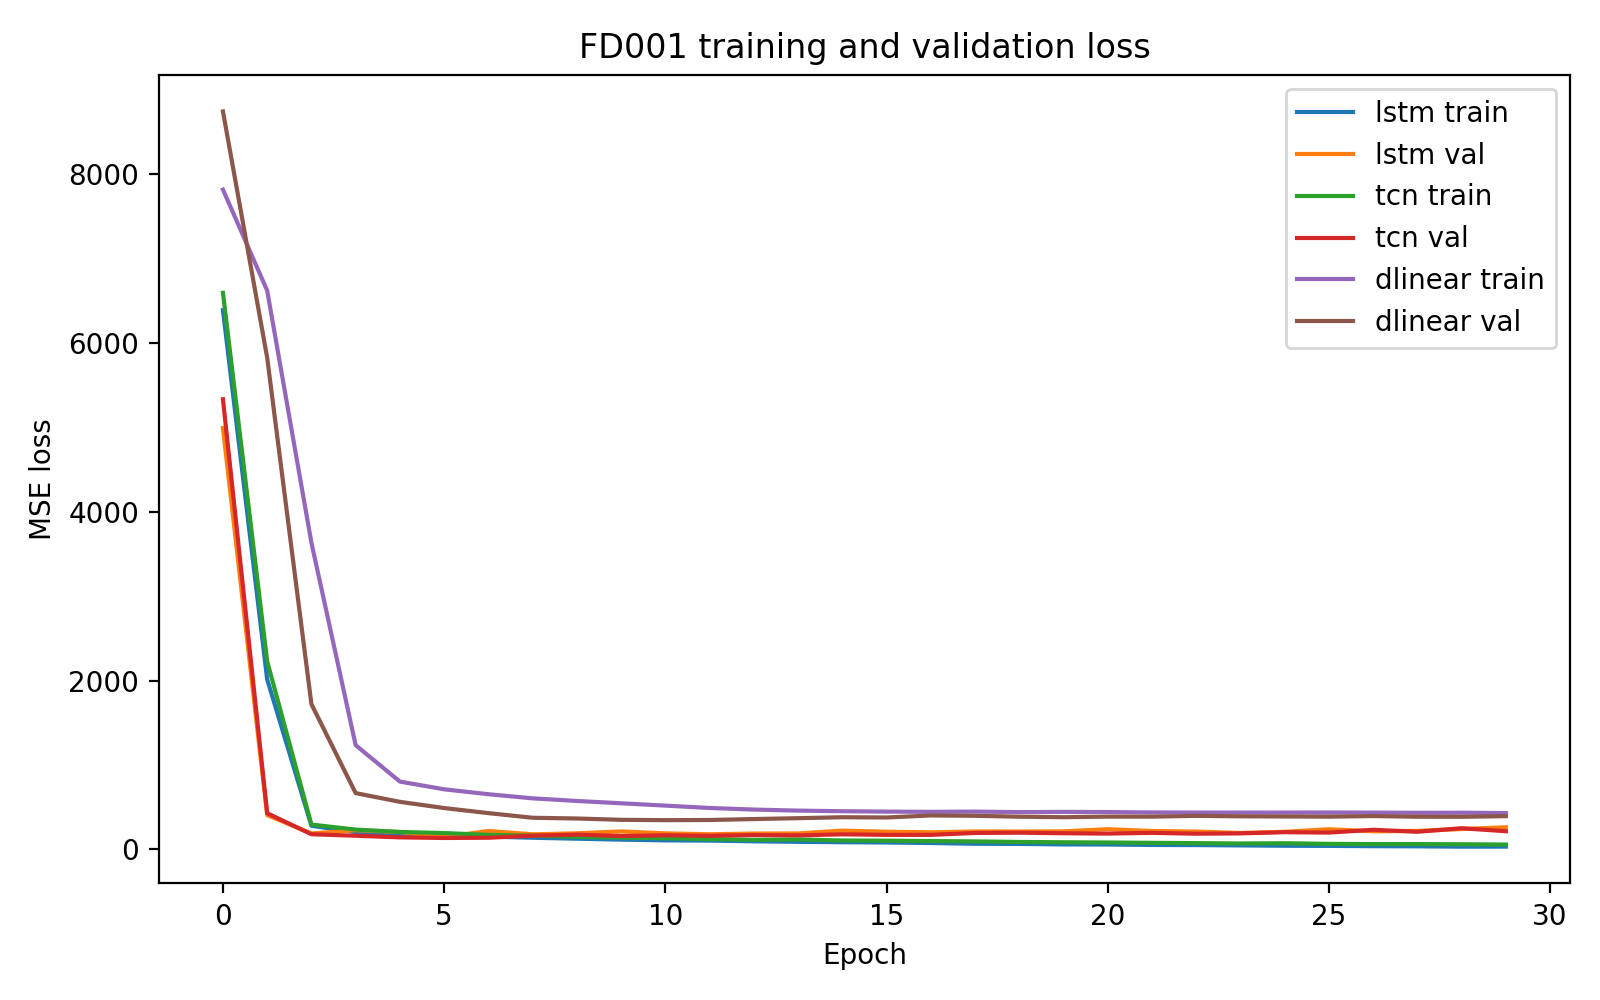
\includegraphics[width=0.78\linewidth]{outputs/FD001/figures/loss_curves.png}
\caption{FD001 training and validation loss curves for the LSTM baseline and two variants.}
\label{fig:fd001_loss}
\end{figure}

\begin{figure}[h]
\centering
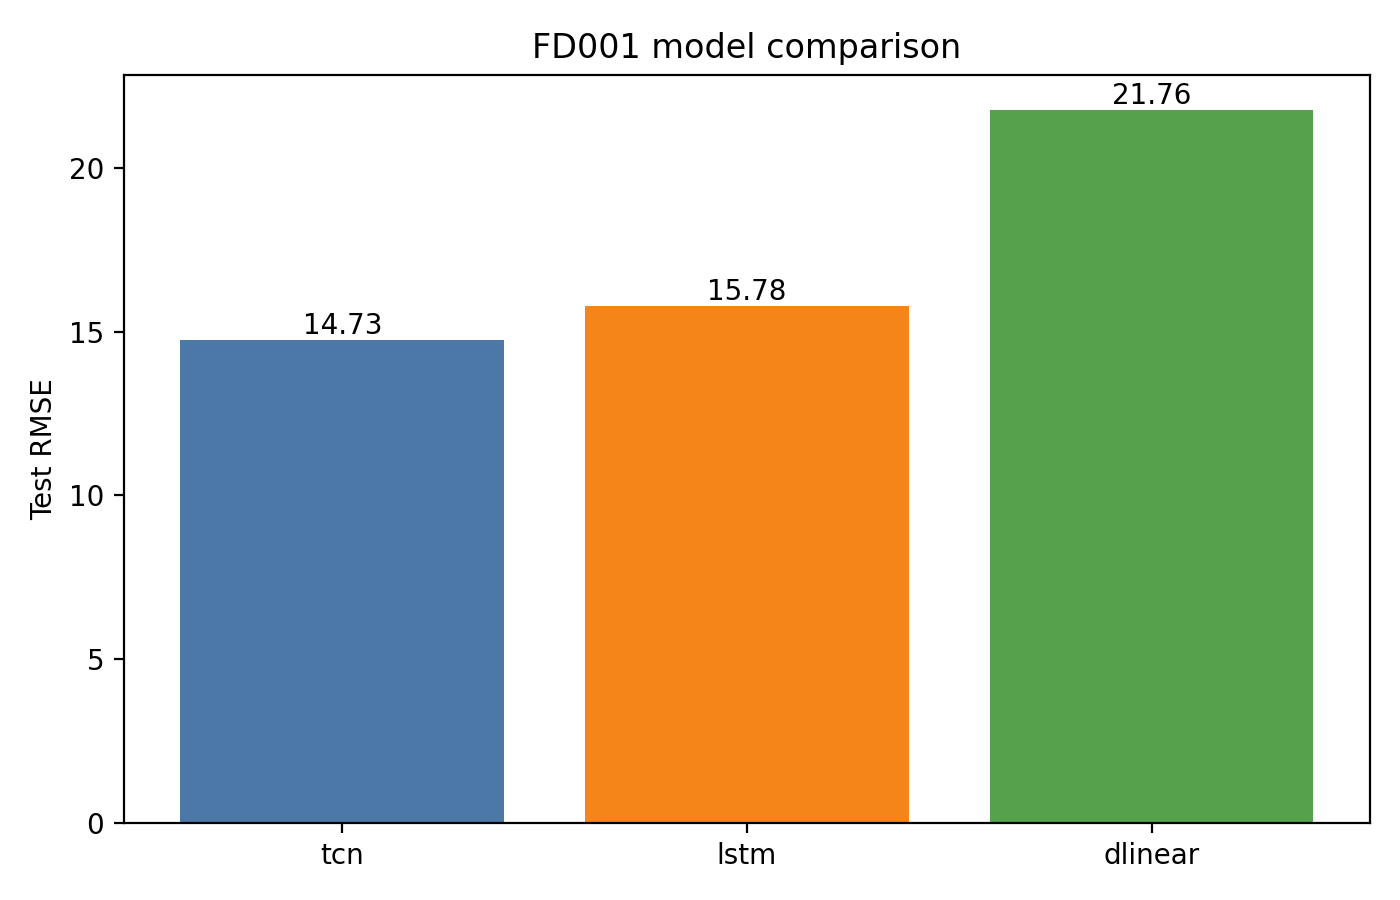
\includegraphics[width=0.68\linewidth]{outputs/FD001/figures/model_rmse_comparison.png}
\caption{FD001 test RMSE comparison. TCN performs best on this easiest subset.}
\label{fig:fd001_rmse}
\end{figure}

Table~\ref{tab:fd001} gives the FD001 metrics. The TCN improves RMSE over the LSTM by about 1.05 cycles and also has the lowest PHM score. This supports the hypothesis that convolutional temporal modeling can be effective when the operating condition is fixed. The DLinear-style model trains fastest and has only 943 trainable parameters, but its RMSE is much higher, suggesting that this task requires more than a simple trend/residual linear model.

\begin{table}[h]
\centering
\caption{FD001 results. Lower RMSE and PHM score are better.}
\label{tab:fd001}
\begin{tabular}{lrrrr}
\toprule
Model & Params & Time (s) & RMSE & PHM \\
\midrule
LSTM & 25,281 & 16.76 & 15.78 & 820.81 \\
TCN & 35,361 & 29.85 & 14.73 & 413.71 \\
DLinear & 943 & 10.43 & 21.76 & 1026.08 \\
\bottomrule
\end{tabular}
\end{table}

\subsection{Full C-MAPSS Subset Analysis}

To make the experiment more complete, I also evaluated all three models on FD002, FD003, and FD004. This is a useful stress test because the later subsets include more operating conditions and fault modes. Table~\ref{tab:all_results} shows the test RMSE across all subsets.

\begin{table}[h]
\centering
\caption{Test RMSE on all C-MAPSS subsets. Lower is better.}
\label{tab:all_results}
\begin{tabular}{lrrr}
\toprule
Subset & LSTM & TCN & DLinear \\
\midrule
FD001 & 15.78 & \textbf{14.73} & 21.76 \\
FD002 & \textbf{15.41} & 16.05 & 20.21 \\
FD003 & \textbf{13.27} & 15.30 & 16.02 \\
FD004 & \textbf{17.19} & 19.87 & 25.31 \\
\bottomrule
\end{tabular}
\end{table}

The LSTM performs best on FD002, FD003, and FD004. This partially contradicts my expectation that the TCN would be consistently stronger. One possible explanation is that the recurrent hidden state gives the LSTM a useful way to summarize degradation history even with a short 30-cycle window. The TCN may need more careful hyperparameter tuning or longer windows to consistently outperform the baseline. The DLinear-style model is smallest and fastest but does not match the nonlinear models, especially on FD004.

FD004 is the hardest subset by design, and it also shows the largest gap between the LSTM and DLinear-style model. This makes sense because FD004 combines multiple operating conditions with multiple fault modes. A simple decomposition model may not separate operating-condition effects from degradation effects as well as the LSTM.

\subsection{Feature Occlusion Analysis}

Figure~\ref{fig:fd004_importance} shows the sensor occlusion analysis for the LSTM on FD004. The most important channels include sensor 11, operating setting 2, sensor 1, sensor 8, and sensor 4. Occluding these features causes a large RMSE increase, which suggests that the model relies heavily on both operating condition variables and specific sensor channels when the subset contains multiple conditions. This is consistent with the dataset description: operating conditions significantly affect the sensor readings in FD002 and FD004.

\begin{figure}[h]
\centering
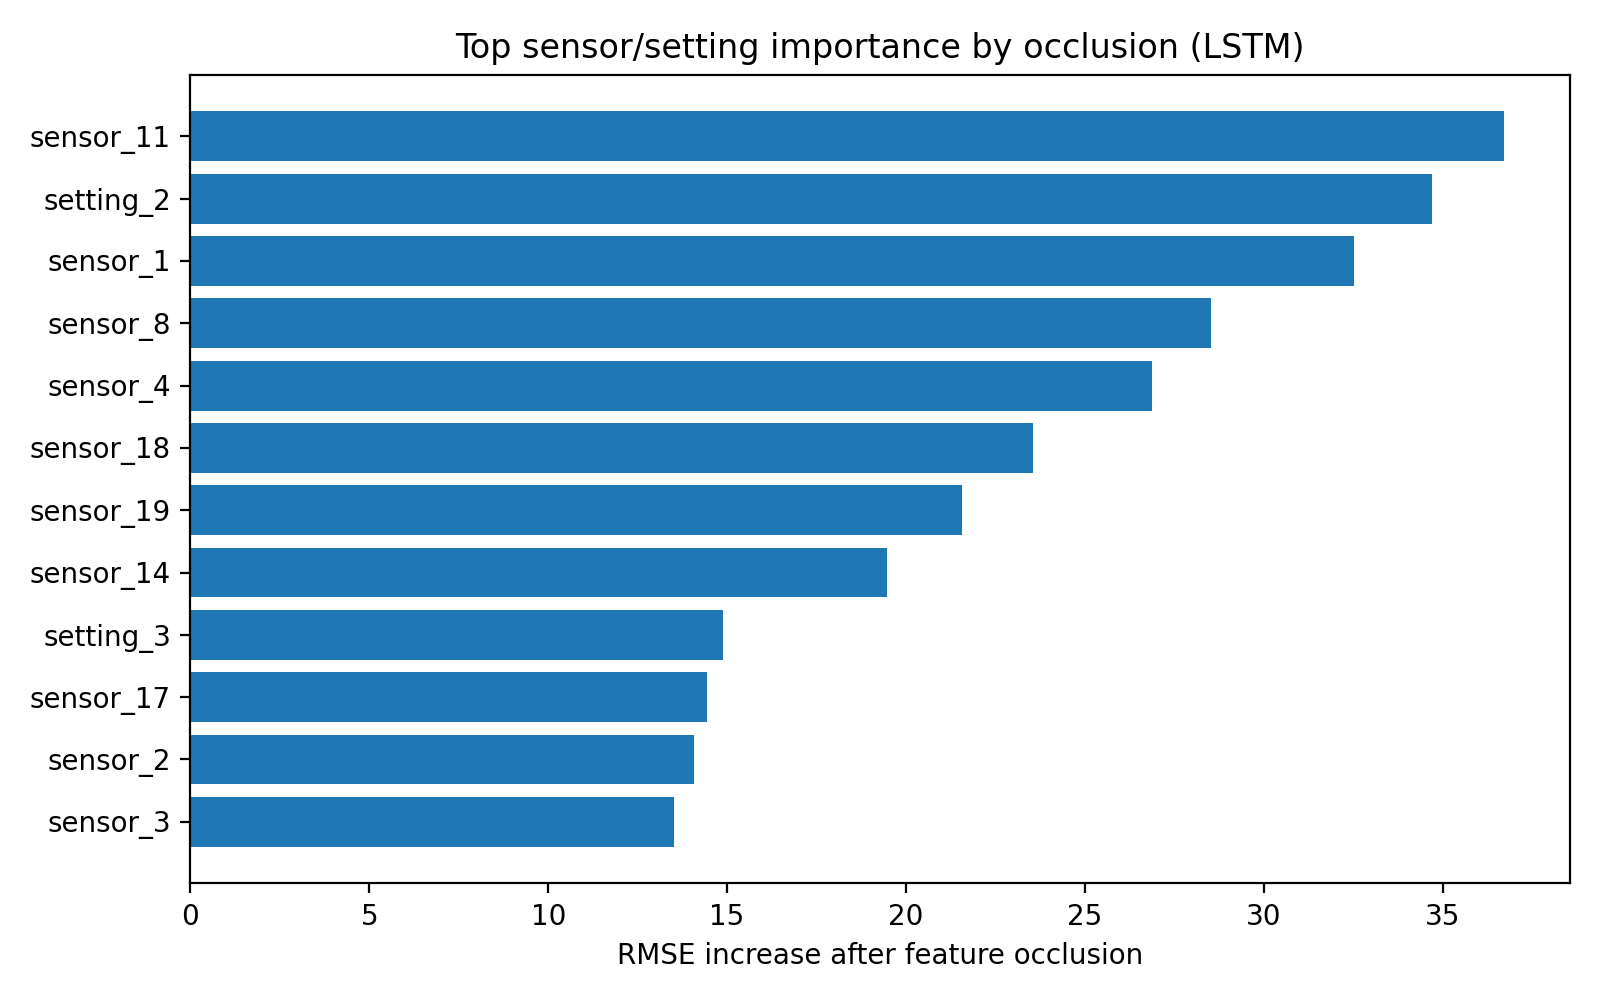
\includegraphics[width=0.82\linewidth]{outputs/FD004/figures/feature_importance_occlusion.png}
\caption{FD004 LSTM feature occlusion analysis. Features are ranked by RMSE increase after setting that feature to zero in the test windows.}
\label{fig:fd004_importance}
\end{figure}

\section{Conclusion}

This project compared an LSTM baseline with TCN and DLinear-style variants for RUL prediction on C-MAPSS. On FD001, the TCN achieved the best RMSE and PHM score, suggesting that dilated temporal convolutions are effective for the simplest operating setting. Across the full FD001--FD004 analysis, however, the LSTM was more robust and achieved the best RMSE on three of the four subsets. The DLinear-style model was much smaller and faster, but it underperformed the nonlinear models on every subset.

The main takeaway is that model complexity should match the structure of the data. A lightweight linear decomposition model is attractive for speed, but C-MAPSS appears to require nonlinear temporal modeling. Given more time, I would tune the window length, run multiple random seeds, and test architectures that explicitly normalize or condition on operating settings for FD002 and FD004.

\section*{Collaboration Statement}

I completed this project individually. I used AI tools to help scaffold code, debug GitHub/RunPod issues, and improve the organization of the README and report draft. I reviewed the experimental setup, results, figures, and final interpretation myself.

\bibliographystyle{plain}
\bibliography{references}

\end{document}
